\documentclass[12pt]{article}

\usepackage[margin=1in]{geometry}

\usepackage{enumerate}
\usepackage{amsmath}
\usepackage{amssymb}
\usepackage{mathtools}  % amsmath with extensions
\usepackage{amsfonts}  % (otherwise \mathbb does nothing)
\usepackage{graphicx}

\newcommand{\R}{\mathbb{R}}
\newcommand{\K}{\mathbb{K}}
\newcommand{\E}{\mathbb{E}}
\newcommand{\N}{\mathbb{N}}
\newcommand{\Ra}{\Rightarrow}
\newcommand{\ra}{\rightarrow}
\newcommand{\ol}{\overline}
\DeclarePairedDelimiter{\norm}{\lVert}{\rVert} 

\begin{document}
\LaTeX \\
Calculo Avanzado\\
Espacios Normados:\\
Javier Vera

\newpage
\noindent
1) Sea E un espacio normado 

\begin{enumerate}[i.]
	\item Las funciones:
		\begin{center}
		$+: \E \times \E \mapsto \E \quad \quad  \times : \K \times \E \mapsto \E$
		\end{center}
	son continuas

		Sean 

		$(x_{n})_{n \in \N} \in \E   \hspace{4pt}/ x_{n}  \ra x \quad \quad  (y_{n})_{n \in \N} \in \E  \hspace{4pt}/ y_{n} \ra y$

		$ \norm {(x_{n} + y_{n}) - (x + y)} \leq \norm {x_{n} - x} - \norm {y_{n}-y} \ra 0 \quad$ luego $\quad  (x_{n} + y_{n}) \ra (x + y)$

		$+ (x_{n},y_{n}) = x_{n} + y_{n} \ra x + y = +(x,y)$

		$\Ra +(x_{n},y_{n}) \ra +(x,y)$

		Sea $\lambda \in \K \quad$ $ (x_{n})_{n\in \N} \in \E \quad x_{n} \ra x$

		Entonces por ser sucesión $\lambda x_{n} \ra \lambda x$

		Luego $\times(\lambda,x_{n}) = \lambda x_{n} \ra \lambda x = \times (\lambda,x) $

		


	\item $\overline {B_{r}(x)} = \overline B_{r}(x)$ (La clausura de una bola abierta de E es la bola cerrada correspondiente)

		$ \overline B(r,x)$ es cerrado y $ B(r,x) \subseteq \overline B(r,x)$ 

		y $\overline {B(r,x)}$ es el cerrado mas pequeño que contiene a $B(r,x)$ 

		$\Ra \overline{B(r,x)} \subseteq \overline B(r,x)$

		Sea $y \in \ol B(r,x)$ Tomo $y_{n} = x + (1-\frac{1}{n}) (y - x) \Ra y_{n} \ra y $

		$\norm{y_{n} - x } = \norm {(1-\frac{1}{n})(y-x)} =  |(1-\frac{1}{n})| \norm {y-x } \leq \norm {y-x} < r $ 

		$ y_{n} \in B(x,r) \quad \forall n \in \N \Ra y \in \ol{B(r,x)}$

		$\Ra \ol B(r,x) = \ol {B(r,x)}$

			

	\item  Si $\E$ tiene dimension positiva, entonces para todo $r<0$ y todo $x\in\E$ es $diam (B_{r}(x)) = 2r$
	
		Sean $ z,y \in B(r,x) \quad \norm {z-x} \leq r \quad \norm {x-y} \leq r$  

		$\Ra \norm {z-y} \leq \norm {z-x} + \norm {x-y} \leq 2r $

		Con la distancia dada por la norma sabemos $d(z,y) \leq 2r \quad \forall x,y \in B(r,x)$ por lo que $2r$ es cota superior de las distancias 

		Resta ver que es la menor de las cotas, supongamos que no lo es:

		 $\Ra \exists \delta \in \R \quad $con$ \quad  \delta \leq r \Ra 2 \delta \leq 2r \quad/ \quad d(x,y) \leq 2\delta $

		 Considerando $ \delta \leq l \leq r \quad $ Sea$  \quad  z \in \E \times \E / \quad z = x + l\frac{x}{\norm {x}}$ y $\quad z' = x - l\frac{x}{\norm{x}}$


		 Sin embargo $\norm {z-z'} = 2r $ por lo que $d(z,z')>2\delta$ abs!

		 Efectivamente 2r era cota superior y menor de las cotas superiores

		 $\Ra sup(d(x,y))=2r \quad \forall x,y \in B(r,x) $

		 $\Ra diam(B(r,x))=2r$


\end{enumerate}

\newpage
\noindent \\
2) Sea $(E,\norm{\cdot})$ un espacio normado y sea $C \subset E$ Decimos que $C$ es $convexo$ si $\forall x,y \in C$ y $\forall t \in [0,1]$ se tiene que $tx + (1-t)y \in C$

\begin{enumerate}[i)]
	\item Probar que $B(r,x)$ es convexo
		\begin{itemize}
			\item Sean $z,y \in B(r,x)$

			\item $ \norm{tz + (1-t)y -x }\leq \norm {tz - tx + tx +y -ty -x} \leq t\norm{(z-x)} + (1-t)\norm{(y-x)} \leq tr + (1-t)r = r$
	
			\item  $ \norm{tz + (1-t)y - x } = r$


		\end{itemize}
			 $\Ra tz + (1-t)y \in B(r,x) \quad \forall x,y \in B(r,x) \quad \forall t \in [0,1]$

		

	\item Probar que si $(C_{i})_{i \in I}$ son convexos entonces $ \bigcap_{i \in I} C_{i}$ lo es

		Sean $z,y \in \bigcap_{i \in I} C_{i} $

		$z,y \in C_{i} \quad $convexo$ \quad \forall i \in I $

		$ tz + (1-t)y \in C_{i} \quad \forall i \in I \quad \forall t \in [0,1]$

		$\Ra tz + (1-t)y \in \bigcap_{i \in I} C_{i} \quad \forall z,y \in \bigcup_{i \in I} C_{i} \quad \forall t \in [0,1]$
	\item Probar que si $C$ es convexo entonces $C^\mathrm{o}$ lo es
		
		\begin{itemize}
			\item Sean $x,y \in C^\mathrm{o} \subseteq C \Ra  \exists B(r_{1},x) \subseteq C \quad B(r_{2},y) \subseteq C $
			\item Como C es convexo se que $tx + (1-t)y \in C$

			\item Ahora afirmo que ademas $tx + (1-t)y \in C^\mathrm{0}$

			\item Sea $t=0$ o $t=1$ Esto es evidente

			\item Si no, tomo un $l \in tx + (1-t)y$ y considero $B(r_{3},l)$ con $r_{3} \leq \inf \{r_{1},r_{2}\}$

		 	\item Ahora afirmo que $B(r_{3},l) \subseteq C$

			\item Dado un $l' \in B(r_{3},l)$ se que $ v = l' - l$ y $ v \in B(r_{3},0)$

			\item $v + x \subseteq B(r_{3},0) + x = B(r_{3},x) \subseteq B(r_{1},x)$ análogo con $y$

			\item Por lo tanto si tomo $x' = x + v \in B(r_{1},x) \subseteq C $ e $y'= y + v \in B(r_{2}, y) \subseteq C$

			$\Ra x',y' \in C$ además puedo afirmar que $l' \in tx' + (1-t)y' $ dado que esta recta es un desplazamiento dado por $v$ de la anteriór recta, como la anteriór tenía a $l$ esta va a tener a $l+v$ y sabemos $l+v=l'$
				
			\item Y sabemos que C es convexo por lo que $ tx' + (1-t)y' \in C \Ra l' \in C$

			\item Luego $B(r_{3},l) \subseteq C$ entonces $l \in C^\mathrm{o}$

			\item $tx + (1-t)y \in C^\mathrm{o} \quad \forall x,y \in C^\mathrm{o} \quad \forall t \in [0,1]$

			$\Ra C^\mathrm{o}$ es convexo

		\end{itemize}
\begin{figure}[ht!]
	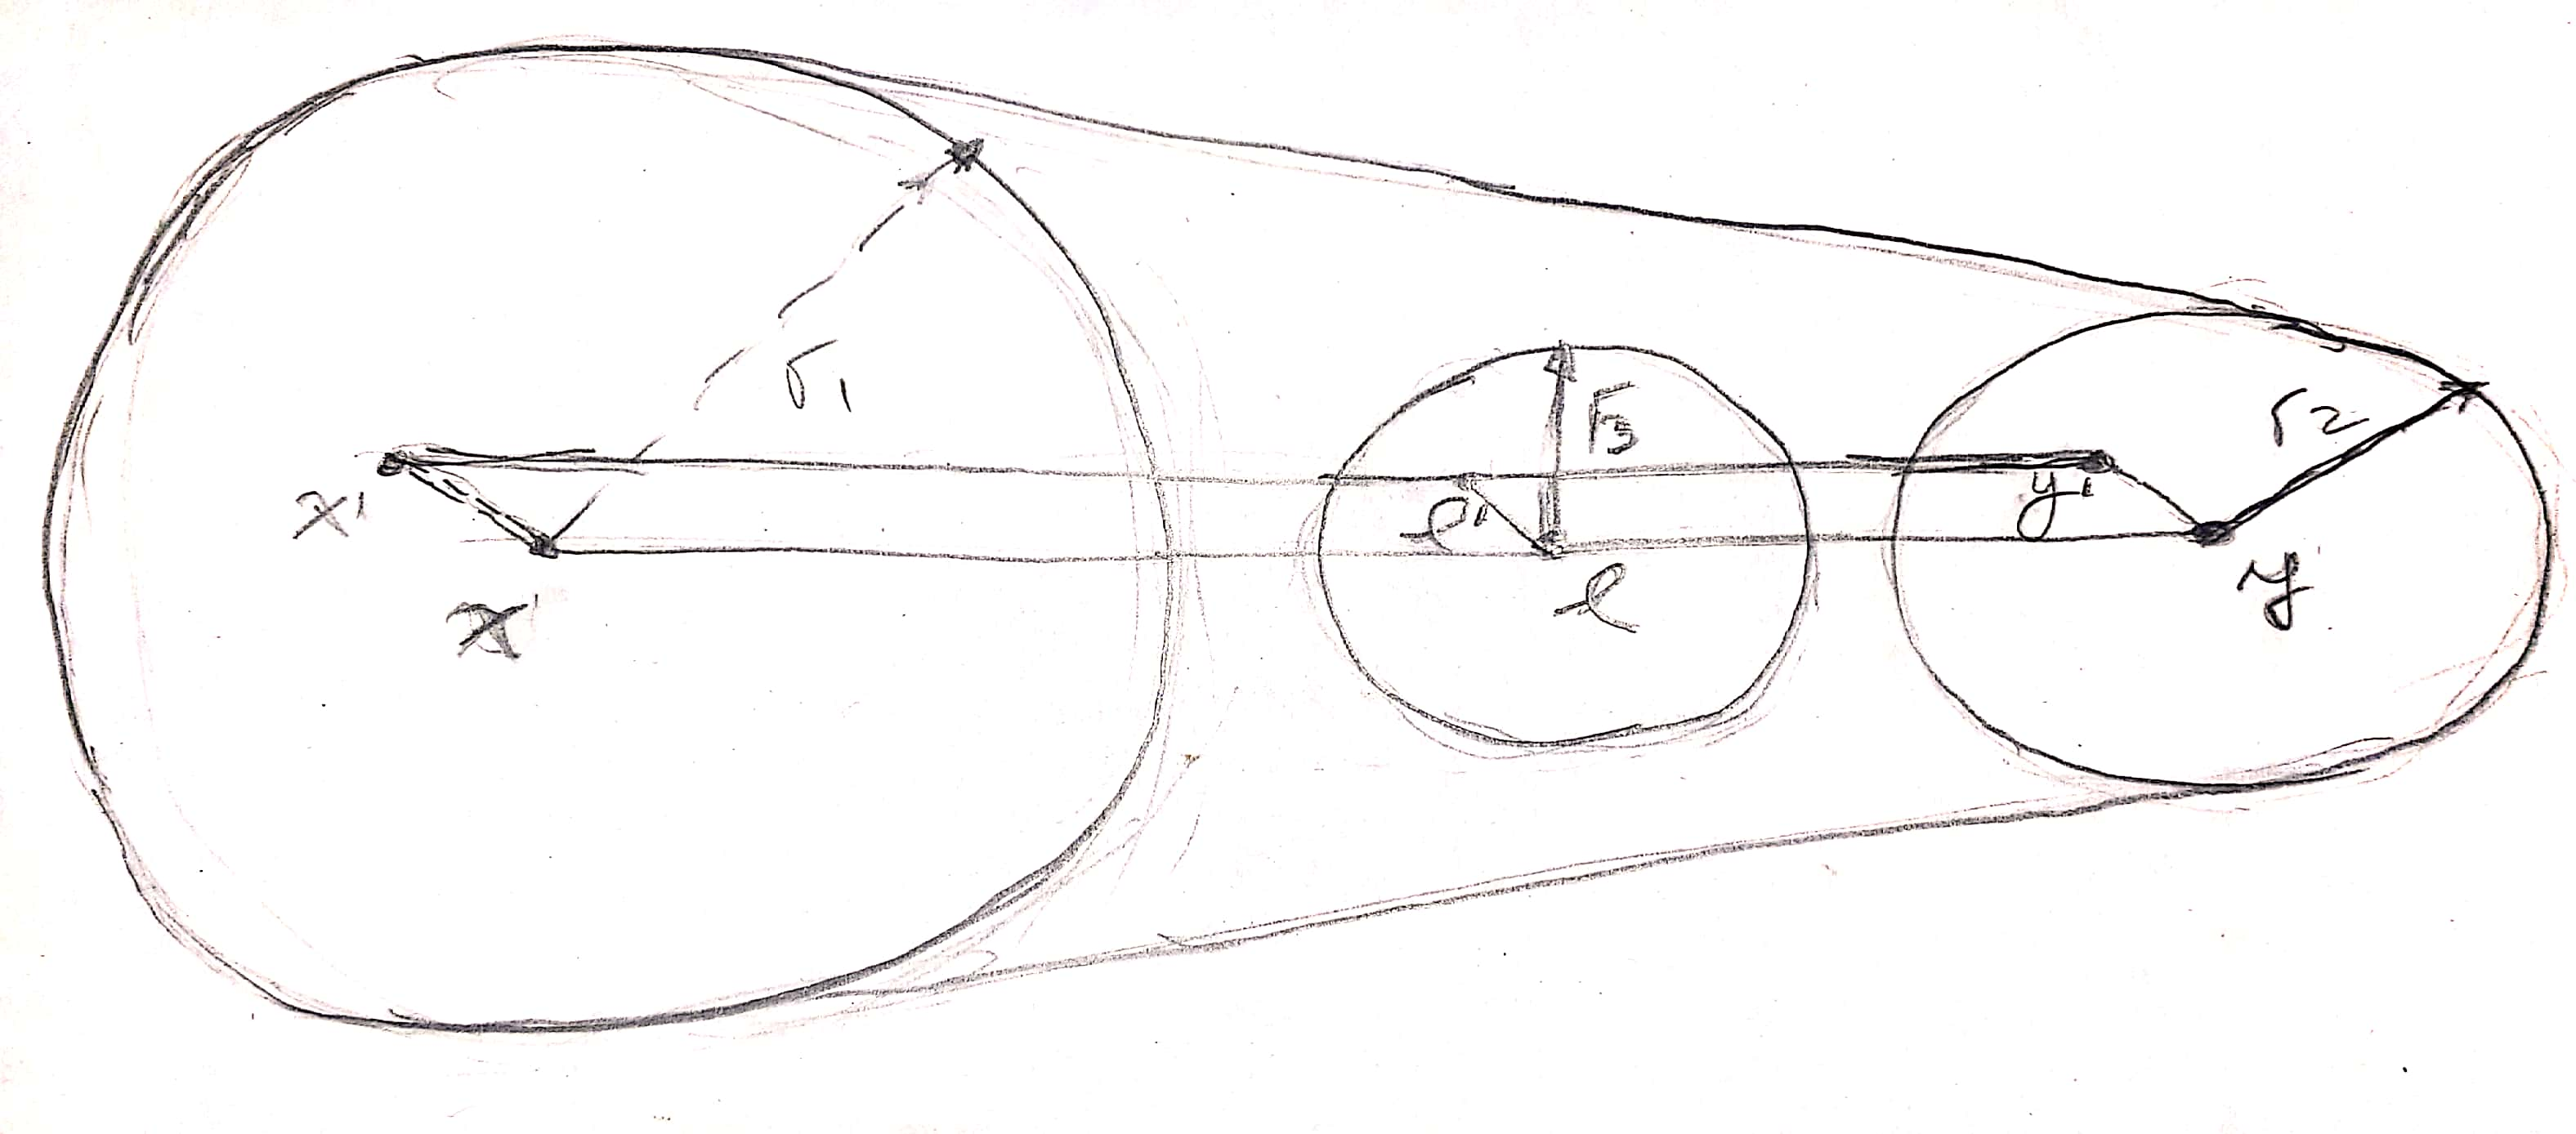
\includegraphics[width=\linewidth]{image.jpg}
	\caption{Ilustración}		
\end{figure}
\end{enumerate}

\newpage
\noindent
\\
iv) Probar que si $C$ es convexo entonces $\ol C$ lo es
\begin{itemize}
	\item Sean $x,y \in \ol C$ se que $ \exists (x_{n})_{n\in \N} \subseteq C $ tq $x_{n} \ra x$ y $\exists (y_{n})_{n\in\N} \subseteq C$ tq $  y_{n} \ra  y$

	\item Luego se que $\norm {tx + (1-t)y - (tx_{n} + (1-t)y_{n})} = \norm {(x-x_{n}) + (1-t)(x-y_{n})} \leq t\norm{(x-x_{n})} + (1-t)\norm{(y-y_{n})} \leq t\epsilon + (1-t) \epsilon = \epsilon \quad \forall n \geq n_{0} \quad \forall t\in [0,1]$

	\item Ademas sabemos que $tx_{n} + (1-t)y_{n} \in C \quad \forall n \in \N$ por que $C$ es convexo

	\item Entonces $tx + (1-t)y \in \ol C \quad \forall x,y \in \ol C \quad \forall t \in [0,1]$

	$\Ra \ol C$ es convexo
\end{itemize}

\noindent
3) Sea $(E,\norm{\cdot})$ un espacio normado y $S \subset E$ un subespacio (vectorial). Probar que:

\begin{enumerate}[i.]

	\item $\ol S$ tambien lo és
		\begin{itemize}
			\item Sean $x,y \in \ol S \quad \exists (x_{n})_{n} \in S , (y_{n})_{n}  \in S$ con $x_{n} \ra x \quad y_{n} \ra y$

			\item Dado que la suma y multiplicacion por escalares son continuas por ser $S$ espacio normado $x_{n} + y_{n} \ra x + y$ y como $S$ subespacio vectorial $(x_{n} + y_{n})_{n} \subseteq S$

			$\Ra x+y \in \ol S$

			\item De la misma forma veo que $\lambda x \in \ol S$

			$\Ra \ol S$ es subespacio

		\end{itemize}

	\item $S \ne E$ entonces $S^\mathrm{o} = \emptyset$

		Supongo $S^\mathrm{o} \neq \emptyset$ entonces $ \exists x \in S^\mathrm{o}$

		Luego $\exists B(r,x) \subseteq S$

		Considero el conjunto $R = \{y - x : y \in B(r,x)\}$ se que $R \subseteq S$ y se que $S = B(r,0)$ 

		Ahora sea $z \in E \setminus \{0\}$ Se que $\frac{r}{2}\frac{z}{\norm{z}} \in B(r,0) \subseteq S$

		Luego $z= \frac{2\norm{z}}{r}.\frac{r}{2}\frac{z}{\norm{z}} $ y como $\frac{2\norm{z}}{r}$ es un escalar y $\frac{r}{2}\frac{z}{\norm{z}} \in S $

		Entonces $ z \in S $ y sabemos que $0 \in S$ por que S es subespacio y $S \subseteq E$

		$\Ra S = E$
		
	\item Si $dim(S) \leq \infty $ entonces $S$ es cerrado

		Supongamos $dim(S)=n$ y consideremos en $S$ la norma inducida por $E$

		Considero el isomorfismo dado por tomar coordenadas $T:S \ra R^n$ (que se que es continuo)

		Ahora si definimos $\norm {x}_{R^n} = \norm{T^{-1}(x)}_{\E}$ entonces es fácil ver que T es en realidad una isometría

		Luego sabemos que $R^n$ es completo para cualquier norma dado que todas sus normas son equivalentes

		$T:S \ra R^n$ es una isometria y ademas tiene inversa por ser un isomorfismo entonces es facil probar que su inversa es tambien una isometria.

		Ahora sabemos que isometrías preservan sucesiones de Cauchy

		Luego dada una sucesion de Cauchy $(a_{n})_{n \in \N} \in S$ se que $T(a_{n})$ tambien es de cauchy

		Entonces $T(a_{n})$ converge por estar en $R^n$ por lo que $S$ es completo

		Otra forma es sabiendo que tener $T$ y $T^{-1}$ ambas isometrías implica que son uniformemente continuas,entonces tenemos un homeomorfismo uniforme , y este preserva completos.

		Por último como $T$ es continua preimagen de convergente es convergente por lo que $T^{-1}(T(a_{n}))$ es convergente

		$\Ra S$ es un completo en $\E$ entonces es cerrado en $\E$

	\item Si $S$ es un hiperplano (osea: $\exists x \neq 0$ tal que $ S
		\oplus <x> = E$) entonces $S$ es o bien denso o bien cerrado en
		$E$

		\begin{itemize}	
			\item Supongo $S$ no es cerrado entonces $\exists x \in \ol S \setminus S $

			\item Luego como $S$ hiperplano $\E = S \oplus <x> \subseteq \ol S \subseteq \E$

			\item $\Ra \E = \ol S$ por lo que $S$ es denso

			\item Ahora supongamos que $S$ es cerrado luego $S = \ol S$

			\item Luego como sabemos que $S \oplus <x> = \ol S \oplus <x> = E$ sabemos que $\exists x \in \E \setminus \ol S$
		
			$\Ra S $ no es denso en $\E$
		\end{itemize}

\end{enumerate}

\noindent 4) Sea $(\E,\norm \cdot)$ un espacio de Banach y $(x_{n})_{n \in \N} \subset \E$. Si $ \sum_{n=1}^{\infty}\norm{x_{n}} $ converge, entonces $\sum_{n=1}^{\infty} x_{n}$
	\begin{itemize}
		\item Como $\sum_{n=1}^{\infty} \norm{x_{n}}$ entonces dado $\epsilon > 0$

		\item $\exists n_{0} $ / $\sum_{n > n_{0}}^{\infty} \norm{x_{n}} \leq \epsilon$

		\item Sea $S_{n} $ la sucesión de sumas parciales de $ \sum_{n=1}^{\infty} x_{n}$
			
		\item Sea $m > n_{0} $ $$\norm{S_{n} - S_{m}} = \norm{\sum_{k=1}^{n} x_{k} - \sum_{k=1}^{m} x_{k} } = \norm{\sum_{m+1}^{n} x_{k}}  = \sum_{m+1}^{n} \norm{x_{k}} \leq \epsilon$$

		\item Luego la sucesión de sumas parciales de la series es de Cauchy, como sabemos que $\E$ es de Banach (completo) y toda sucesión de Cauchy en un completo converge 

		\item $S_{n}$ es de Cauchy y $(S_{n})_{n \in \N} \in \E $ entonces $ S_{n}$ converge

		$\Ra \sum_{n=0}^{\infty} x_{n}$ converge
	\end{itemize}


\noindent 5) Para cada uno de los siguiente ejemplos decidir si son cerrados si son densos y si son hiperplanos:
	\begin{enumerate}[i.]
		\item $c = \{(x_{n})_{n \in \N} : \exists \lim_{n \ra + \infty} x_{n}   \} \subseteq \ell_{\infty}$

			\begin{itemize} 

			\item Voy a ver que $c$ es cerrado.

			\item Sea $(x_{n})_{n \in \N} \in c $ con $x_{n} \ra x_{0}$

			\item $x_{n}^{r} \ra x_{0}^{r}$ y $\norm {x_{n}^{r} - x_{m}^{r}} = \sup_{r \in \N} |x_{n}^{r} - x_{m}^{r}|$
			
			\item Como $x_{n} \ra x_{0}$ sabemos que $\exists n_{0} \in \N $ con $\norm{x_{n}^{r} - x_{0}^{r}} \leq \frac{\epsilon}{3} \quad \forall n>n_{0} $

			\item Por otro lado como $x_{n}^{r}$ es convergente sabemos que es de cauchy

			\item Luego sabemos $x_{n}^{r}$ es una sucesion de sucesiones de $c$ por ende cada una de estas sucesiones converge luego es de cauchy

			\item Entonces fijado un n sabemos que $\exists N \in \N $ / $\norm{x_{n}^{r} - x_{n}^{p}} \leq \frac{\epsilon}{3} \quad \forall r,p > N$

			\item Finalmente $\norm {x_{0}^{r} - x_{0}^{p}} = \norm {x_{0}^{r} - x_{n}^{r} } + \norm {x_{n}^{r} -  x_{n}^{p}} + \norm{x_{n}^{p} - x_{0}^{p}} \leq \frac {\epsilon}{3} + \frac {\epsilon}{3} +  \frac {\epsilon}{3} = \epsilon$

			\item Luego $x_{0}^{r} $ es de cauchy y como $\R$ es completo converge

			\end{itemize}

		\item $c_{0} = \{(x_{n})_{n \in \N} : x_{n} \ra 0 \} \subseteq c$ 

		Usando el mismo argumento que en el i) vemos que es cerrado

			Consideremos $L:c \ra \R$ tal que $L((a_{n})_{n \in \N}) = \lim_{n \ra \infty} a_{n}$

			Esta es una función lineal, continua y no nula y por ende $c_{0} = \ker (L)$ 

			Luego $c_{0}$ es un hiperplano 

			falta ver cerrado

		\item $A = \{x_{n} \in \ell^1\ : \sum_{n=1}^{\infty} x_{n} = 0\} \subseteq \ell^1$

			Sea $(x_{n})_{n \in \N }  \in A $ luego $\sum_{n > 0} |x_{n}| $ es convergente

			Defino $f: \ell^1 \ra \R$ como $x_{n} \ra \sum_{n>0} |x_{n}|$

			Esta función es no nula, y ademas vemos que es continua

			$|f(x_{n})| \leq |\sum_{n>0} x_{n}| \leq \sum_{n>0} |x_{n}| = \norm {x_{n}} $

			Luego $\ker f = A$ entonces $A$ es hiperplano de $\ell^1$
			
			Falta ver crrado

		\item $B = \{x_{n} \in \ell^2\ : \sum_{n=1}^{\infty} x_{n} = 0\} \subseteq \ell^2$



		\item $\R[X] \subseteq C[0,1]$

			Por Weierstrauss-Stone sabemos que $\R [X]$ es denso en $C[0,1]$
			
			Sabemos que hay funciones continuas en el $[0,1]$ que no son polinomios

			Entonces sabemos que no es cerrado, si lo fuera seria $\R[X] = \ol{\R[X]} = C[0,1]$

			No es hiperplano , por ejemplo las funciones $sen$ y $coseno$

		\item $C^1[a,b] \subseteq C[a,b] $

		falta hacer , consultar
	\end{enumerate}

\noindent
6) Si $T: \E \ra F $ es una función lineal entre espacios normados, entonces las siguientes afirmaciones son equivalentes:

	\begin{enumerate}[i.]
			
		\item La función $T$ es continua en 0	

		\item Existe $x_{0} \in \E$ tal que la función $T$ es continua en $x_{0}$

		\item La función $T$ es continua

		\item La función $T$ es uniformemente continua

		\item Existe un número $M>0$ tal que para todo $x \in \E$ es $\norm{T(x)} \leq M\norm{x} $

		\item Para todo subconjunto acotado $A$ de $ \E$ el conjunto $T(A)$ es acotado
	\end{enumerate}
\end{document}




